\SourceLeaf{171}
Gesetzt, $CD$ würde von $CE$ in $F$ geschnitten, so sei $FG$ auf $AB$ senkrecht
und $GFE$ wird $= ACF$ sein, aber $< BEF$. Q[uod]. E[st]. A[bsurdum].

5) Man mache iisdem suppositis $EBH = BEF$, so wird $BH$ die $EC$
nicht schneiden, wohl aber die Parallele $CJ$, welches absurd ist.

\bigskip
\hrule
\bigskip

\begin{center}BEMERKUNGEN.\end{center}

\smallskip

Die vorstehende Notiz findet sich auf der letzten Seite eines Handbuches, das den Titel trägt: Mathematische Brouillons. October 1805. Lässt sich auch die Zeit der Abfassung nicht genau feststellen, so zeigt doch der Inhalt der Notiz, dass sie an den Anfang von \textsc{Gauss}’ Untersuchungen über die ersten Gründe der Geometrie gehört.

Der in 3) angedeutete Beweis beruht auf dem Hülfssatze: Trägt man auf dem einen Schenkel eines Winkels der Grösse
\[
\frac{90^{0}}{2^n}
\]
vom Scheitelpunkte aus die Strecke $2^n.l$ ab, so ist das vom Endpunkte dieser Strecke auf den andern Schenkel gefällte Loth grösser als $l$.

\begin{center}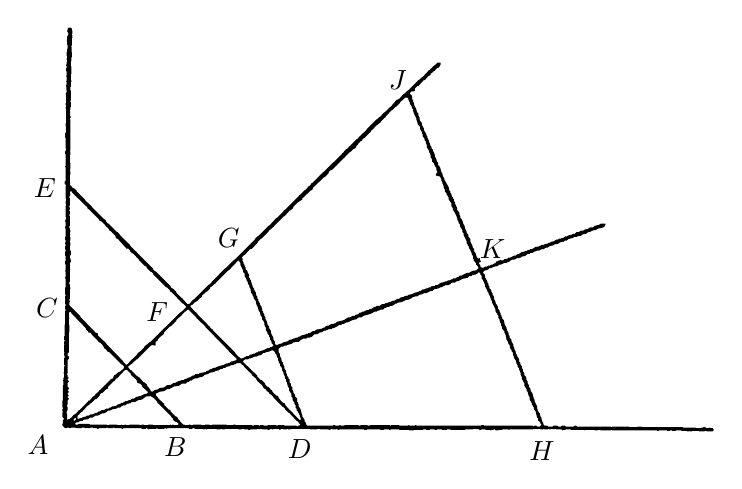
\begin{tikzpicture}[x=0.00672646cm,y=-0.00672646cm]
\fill[even odd rule] (104,73) -- (103,78) -- (105,81) -- (105,84) -- (103,88) -- (103,94) -- (102,95) -- (103,96) -- (103,103) -- (104,104) -- (104,110) -- (103,111) -- (103,116) -- (102,117) -- (102,124) -- (103,125) -- (102,131) -- (103,132) -- (103,135) -- (102,136) -- (102,140) -- (101,141) -- (101,143) -- (102,144) -- (102,147) -- (101,148) -- (101,153) -- (102,154) -- (102,161) -- (101,162) -- (102,164) -- (102,171) -- (101,172) -- (102,174) -- (102,178) -- (101,179) -- (102,193) -- (100,195) -- (101,197) -- (101,212) -- (100,213) -- (100,217) -- (101,218) -- (101,220) -- (100,221) -- (100,223) -- (101,224) -- (101,251) -- (100,252) -- (101,268) -- (99,271) -- (99,278) -- (100,279) -- (100,298) -- (101,299) -- (101,301) -- (99,305) -- (99,309) -- (100,310) -- (100,317) -- (101,319) -- (100,320) -- (100,332) -- (99,333) -- (100,335) -- (100,360) -- (98,362) -- (98,365) -- (101,369) -- (100,371) -- (100,393) -- (101,394) -- (101,397) -- (100,398) -- (100,403) -- (101,404) -- (101,406) -- (100,407) -- (100,428) -- (101,429) -- (101,432) -- (99,436) -- (100,438) -- (100,446) -- (99,447) -- (99,449) -- (100,450) -- (100,465) -- (99,466) -- (99,471) -- (100,472) -- (100,476) -- (99,477) -- (99,479) -- (100,480) -- (100,483) -- (99,484) -- (99,489) -- (100,490) -- (100,493) -- (99,494) -- (99,501) -- (100,502) -- (100,511) -- (99,512) -- (99,517) -- (100,518) -- (100,529) -- (99,530) -- (100,532) -- (100,541) -- (99,542) -- (99,544) -- (100,545) -- (100,561) -- (99,562) -- (99,574) -- (100,575) -- (100,577) -- (99,578) -- (99,583) -- (100,585) -- (99,586) -- (99,592) -- (100,593) -- (100,596) -- (99,597) -- (99,602) -- (100,603) -- (100,605) -- (99,606) -- (99,631) -- (98,632) -- (98,653) -- (97,654) -- (97,660) -- (98,661) -- (98,663) -- (97,664) -- (97,668) -- (98,669) -- (97,671) -- (97,683) -- (98,684) -- (97,686) -- (97,689) -- (98,690) -- (98,694) -- (97,695) -- (97,707) -- (98,708) -- (98,710) -- (97,711) -- (97,721) -- (96,722) -- (97,724) -- (97,731) -- (96,732) -- (96,736) -- (95,737) -- (96,739) -- (96,745) -- (95,746) -- (95,774) -- (94,775) -- (94,787) -- (95,788) -- (95,790) -- (94,791) -- (94,795) -- (95,796) -- (94,798) -- (94,806) -- (97,809) -- (97,810) -- (95,812) -- (95,818) -- (94,819) -- (94,822) -- (99,827) -- (102,827) -- (103,826) -- (106,826) -- (107,827) -- (109,827) -- (110,826) -- (119,826) -- (120,827) -- (130,827) -- (131,826) -- (136,826) -- (137,827) -- (141,826) -- (142,827) -- (146,827) -- (147,826) -- (152,826) -- (153,827) -- (159,827) -- (160,828) -- (162,828) -- (163,827) -- (176,827) -- (177,826) -- (179,826) -- (180,827) -- (189,827) -- (190,826) -- (192,826) -- (193,827) -- (205,827) -- (206,828) -- (208,828) -- (209,827) -- (243,827) -- (244,828) -- (251,828) -- (252,827) -- (254,827) -- (256,829) -- (257,829) -- (258,828) -- (271,828) -- (272,827) -- (274,828) -- (286,828) -- (287,827) -- (291,828) -- (292,827) -- (323,827) -- (325,826) -- (326,827) -- (332,827) -- (333,828) -- (339,828) -- (340,827) -- (343,827) -- (344,828) -- (359,828) -- (360,829) -- (362,829) -- (363,828) -- (365,829) -- (367,829) -- (368,828) -- (384,828) -- (385,829) -- (392,829) -- (393,828) -- (395,828) -- (396,829) -- (400,829) -- (401,828) -- (409,828) -- (410,829) -- (412,828) -- (425,828) -- (426,829) -- (432,829) -- (433,828) -- (436,828) -- (437,829) -- (444,829) -- (445,830) -- (448,830) -- (449,829) -- (461,829) -- (462,828) -- (467,829) -- (468,828) -- (471,828) -- (472,829) -- (481,829) -- (482,830) -- (484,830) -- (488,828) -- (490,829) -- (492,829) -- (493,828) -- (502,828) -- (504,830) -- (505,830) -- (507,828) -- (510,828) -- (511,829) -- (517,829) -- (518,828) -- (520,829) -- (525,829) -- (526,828) -- (561,828) -- (562,829) -- (574,829) -- (575,828) -- (580,828) -- (581,829) -- (596,829) -- (597,830) -- (599,830) -- (601,828) -- (603,829) -- (610,829) -- (612,828) -- (614,830) -- (616,830) -- (617,829) -- (663,829) -- (664,830) -- (668,830) -- (669,829) -- (693,829) -- (694,830) -- (700,830) -- (701,829) -- (710,829) -- (711,830) -- (713,830) -- (714,829) -- (729,829) -- (730,830) -- (748,830) -- (749,831) -- (757,831) -- (758,830) -- (774,830) -- (775,829) -- (780,829) -- (781,830) -- (787,830) -- (788,829) -- (796,829) -- (797,830) -- (800,830) -- (801,829) -- (810,829) -- (811,830) -- (819,830) -- (820,829) -- (826,829) -- (827,830) -- (854,830) -- (855,829) -- (869,829) -- (870,828) -- (880,829) -- (881,830) -- (884,830) -- (885,829) -- (892,829) -- (893,830) -- (901,830) -- (902,831) -- (910,829) -- (912,831) -- (916,831) -- (917,830) -- (924,830) -- (925,829) -- (935,829) -- (937,830) -- (938,829) -- (982,829) -- (983,828) -- (985,829) -- (987,828) -- (989,828) -- (990,829) -- (992,828) -- (995,828) -- (996,829) -- (1001,829) -- (1002,828) -- (1004,829) -- (1010,829) -- (1011,828) -- (1013,829) -- (1015,829) -- (1016,828) -- (1022,829) -- (1023,828) -- (1025,828) -- (1026,829) -- (1036,829) -- (1038,831) -- (1040,830) -- (1043,830) -- (1044,829) -- (1053,829) -- (1054,830) -- (1078,830) -- (1079,831) -- (1081,830) -- (1098,830) -- (1099,831) -- (1104,831) -- (1105,830) -- (1109,830) -- (1110,831) -- (1129,831) -- (1130,830) -- (1132,831) -- (1216,831) -- (1217,832) -- (1219,832) -- (1220,831) -- (1235,831) -- (1236,832) -- (1240,832) -- (1241,831) -- (1244,831) -- (1245,832) -- (1251,832) -- (1252,831) -- (1262,831) -- (1263,832) -- (1272,832) -- (1273,833) -- (1276,833) -- (1277,832) -- (1278,833) -- (1282,833) -- (1283,832) -- (1295,832) -- (1296,833) -- (1306,833) -- (1307,832) -- (1309,832) -- (1310,833) -- (1321,833) -- (1323,831) -- (1323,829) -- (1321,827) -- (1318,827) -- (1317,826) -- (1315,826) -- (1314,827) -- (1310,827) -- (1307,825) -- (1304,825) -- (1303,826) -- (1300,826) -- (1299,827) -- (1290,827) -- (1289,826) -- (1266,826) -- (1265,825) -- (1188,825) -- (1187,824) -- (1185,824) -- (1184,825) -- (1183,824) -- (1180,824) -- (1179,825) -- (1164,825) -- (1163,824) -- (1132,824) -- (1130,825) -- (1129,824) -- (1065,824) -- (1063,822) -- (1061,822) -- (1059,824) -- (1044,824) -- (1042,822) -- (1037,822) -- (1035,824) -- (1030,824) -- (1028,822) -- (1021,822) -- (1019,824) -- (1011,824) -- (1009,822) -- (1004,822) -- (1002,820) -- (1001,816) -- (999,813) -- (998,807) -- (996,804) -- (995,799) -- (993,797) -- (991,793) -- (991,791) -- (990,790) -- (990,786) -- (985,776) -- (985,773) -- (984,772) -- (981,761) -- (978,757) -- (977,752) -- (975,750) -- (974,745) -- (972,742) -- (972,739) -- (970,736) -- (969,730) -- (966,727) -- (966,724) -- (963,719) -- (963,716) -- (961,713) -- (961,710) -- (959,708) -- (958,703) -- (956,701) -- (956,697) -- (954,693) -- (952,691) -- (952,689) -- (950,686) -- (949,681) -- (947,678) -- (947,676) -- (945,672) -- (945,669) -- (942,664) -- (941,659) -- (938,656) -- (938,653) -- (936,650) -- (936,647) -- (933,642) -- (932,637) -- (929,632) -- (927,623) -- (924,620) -- (924,618) -- (923,617) -- (923,615) -- (921,613) -- (921,610) -- (919,607) -- (919,605) -- (916,601) -- (916,598) -- (914,594) -- (912,592) -- (911,587) -- (909,584) -- (909,580) -- (906,575) -- (906,573) -- (904,570) -- (903,566) -- (900,563) -- (900,559) -- (898,557) -- (898,554) -- (896,552) -- (896,550) -- (892,543) -- (891,537) -- (888,534) -- (888,532) -- (891,529) -- (894,529) -- (898,527) -- (900,525) -- (903,525) -- (909,522) -- (915,521) -- (919,518) -- (922,518) -- (928,515) -- (932,515) -- (935,513) -- (937,513) -- (939,511) -- (943,509) -- (946,509) -- (952,506) -- (956,506) -- (957,505) -- (959,505) -- (961,503) -- (967,502) -- (972,498) -- (976,498) -- (977,496) -- (981,496) -- (986,493) -- (988,493) -- (989,492) -- (993,492) -- (999,489) -- (1002,489) -- (1007,486) -- (1010,486) -- (1014,483) -- (1020,482) -- (1023,480) -- (1029,479) -- (1034,476) -- (1040,475) -- (1042,473) -- (1045,473) -- (1049,470) -- (1057,468) -- (1060,466) -- (1064,466) -- (1068,464) -- (1072,464) -- (1076,461) -- (1082,460) -- (1086,457) -- (1091,456) -- (1094,454) -- (1100,453) -- (1106,450) -- (1115,448) -- (1118,445) -- (1119,442) -- (1118,441) -- (1110,441) -- (1107,443) -- (1099,445) -- (1095,448) -- (1090,448) -- (1085,451) -- (1080,452) -- (1077,454) -- (1073,454) -- (1068,457) -- (1064,457) -- (1061,460) -- (1058,460) -- (1055,462) -- (1049,463) -- (1046,465) -- (1043,465) -- (1039,468) -- (1036,468) -- (1035,469) -- (1032,469) -- (1029,471) -- (1026,471) -- (1022,474) -- (1017,475) -- (1014,477) -- (1011,477) -- (1009,479) -- (1006,479) -- (1002,481) -- (999,481) -- (993,484) -- (986,485) -- (984,487) -- (980,489) -- (977,489) -- (975,491) -- (972,491) -- (971,492) -- (960,495) -- (956,498) -- (952,499) -- (950,501) -- (947,501) -- (939,505) -- (936,505) -- (934,507) -- (928,508) -- (926,510) -- (922,510) -- (921,509) -- (920,510) -- (918,510) -- (915,512) -- (913,512) -- (911,516) -- (909,516) -- (906,518) -- (903,518) -- (901,520) -- (898,520) -- (895,522) -- (892,522) -- (889,524) -- (885,524) -- (883,522) -- (883,520) -- (880,516) -- (880,515) -- (882,513) -- (884,513) -- (882,509) -- (882,507) -- (881,506) -- (879,507) -- (876,504) -- (874,497) -- (871,493) -- (871,489) -- (868,485) -- (868,483) -- (864,475) -- (864,470) -- (860,465) -- (860,462) -- (857,458) -- (857,456) -- (854,450) -- (853,445) -- (850,440) -- (850,438) -- (847,432) -- (845,430) -- (845,427) -- (843,423) -- (843,420) -- (839,415) -- (839,411) -- (837,408) -- (837,406) -- (835,404) -- (835,401) -- (833,398) -- (833,395) -- (831,393) -- (831,391) -- (829,389) -- (828,385) -- (826,383) -- (826,380) -- (824,378) -- (823,372) -- (815,358) -- (815,356) -- (812,351) -- (811,346) -- (809,343) -- (807,335) -- (803,330) -- (803,326) -- (801,324) -- (799,317) -- (797,315) -- (797,311) -- (796,310) -- (796,308) -- (793,303) -- (793,301) -- (791,299) -- (790,295) -- (788,293) -- (788,290) -- (786,287) -- (786,285) -- (783,279) -- (783,277) -- (781,274) -- (781,272) -- (776,264) -- (776,261) -- (773,255) -- (772,250) -- (770,248) -- (768,244) -- (768,241) -- (766,237) -- (766,233) -- (763,230) -- (762,225) -- (758,217) -- (758,214) -- (756,211) -- (756,208) -- (754,206) -- (754,200) -- (750,196) -- (750,194) -- (753,191) -- (758,191) -- (759,190) -- (759,186) -- (764,181) -- (766,181) -- (776,170) -- (778,170) -- (784,163) -- (789,160) -- (789,158) -- (790,157) -- (791,157) -- (795,153) -- (796,153) -- (801,147) -- (803,147) -- (806,144) -- (808,140) -- (808,138) -- (807,137) -- (802,137) -- (797,142) -- (796,142) -- (787,151) -- (786,151) -- (774,164) -- (773,164) -- (768,169) -- (767,169) -- (746,190) -- (745,190) -- (739,196) -- (738,196) -- (730,205) -- (729,205) -- (727,207) -- (725,207) -- (713,221) -- (712,221) -- (702,231) -- (701,231) -- (693,240) -- (692,240) -- (688,244) -- (687,244) -- (668,263) -- (668,264) -- (653,278) -- (653,279) -- (651,281) -- (650,281) -- (636,295) -- (635,295) -- (634,297) -- (631,300) -- (630,300) -- (625,305) -- (625,306) -- (623,308) -- (622,308) -- (621,310) -- (581,349) -- (580,349) -- (579,351) -- (566,364) -- (565,364) -- (563,366) -- (563,367) -- (560,370) -- (559,370) -- (553,377) -- (552,377) -- (542,387) -- (541,387) -- (540,389) -- (514,415) -- (513,415) -- (511,417) -- (511,418) -- (499,430) -- (498,430) -- (485,444) -- (484,444) -- (464,464) -- (463,464) -- (457,470) -- (457,471) -- (419,509) -- (418,509) -- (402,525) -- (401,525) -- (371,556) -- (370,556) -- (342,584) -- (341,584) -- (333,593) -- (330,593) -- (322,584) -- (322,583) -- (320,582) -- (309,571) -- (309,570) -- (302,563) -- (301,563) -- (298,560) -- (298,559) -- (270,531) -- (269,531) -- (265,527) -- (265,526) -- (234,495) -- (234,494) -- (232,493) -- (223,484) -- (220,479) -- (218,478) -- (202,462) -- (202,461) -- (198,457) -- (197,457) -- (181,441) -- (180,441) -- (177,438) -- (176,435) -- (174,433) -- (173,433) -- (149,409) -- (149,408) -- (137,397) -- (137,396) -- (121,380) -- (121,379) -- (117,375) -- (113,373) -- (108,367) -- (108,365) -- (109,364) -- (108,363) -- (108,349) -- (109,348) -- (109,342) -- (108,341) -- (108,339) -- (109,338) -- (109,326) -- (108,325) -- (108,320) -- (109,319) -- (108,317) -- (108,312) -- (109,311) -- (109,305) -- (108,304) -- (109,303) -- (108,302) -- (109,301) -- (109,245) -- (108,244) -- (108,242) -- (110,240) -- (108,236) -- (108,233) -- (109,232) -- (108,227) -- (109,226) -- (109,221) -- (110,220) -- (110,212) -- (109,211) -- (109,209) -- (110,208) -- (110,190) -- (109,189) -- (109,183) -- (110,182) -- (110,174) -- (111,173) -- (111,171) -- (110,170) -- (110,159) -- (111,158) -- (111,145) -- (110,144) -- (110,135) -- (111,134) -- (111,127) -- (112,126) -- (111,105) -- (112,104) -- (112,91) -- (113,90) -- (113,86) -- (112,85) -- (112,83) -- (113,82) -- (113,77) -- (112,76) -- (112,73) -- (110,71) -- (106,71) -- cycle
(118,807) -- (120,809) -- (120,810) -- (117,813) -- (116,813) -- (115,812) -- (115,810) -- cycle
(313,818) -- (313,820) -- (312,821) -- (304,821) -- (303,820) -- (301,821) -- (299,821) -- (298,820) -- (296,821) -- (265,821) -- (264,820) -- (256,820) -- (255,821) -- (248,821) -- (247,820) -- (244,820) -- (243,821) -- (240,821) -- (239,820) -- (221,820) -- (220,821) -- (215,821) -- (214,820) -- (212,820) -- (211,821) -- (207,821) -- (206,820) -- (204,821) -- (198,821) -- (197,820) -- (183,820) -- (182,821) -- (179,821) -- (178,820) -- (146,820) -- (145,819) -- (124,819) -- (123,820) -- (119,820) -- (118,819) -- (118,818) -- (120,816) -- (123,816) -- (126,814) -- (132,813) -- (134,811) -- (142,810) -- (146,807) -- (150,807) -- (157,803) -- (161,803) -- (169,799) -- (172,799) -- (178,796) -- (180,794) -- (183,794) -- (189,791) -- (196,790) -- (198,788) -- (203,788) -- (205,786) -- (209,784) -- (212,784) -- (216,781) -- (222,780) -- (224,778) -- (232,777) -- (237,774) -- (244,773) -- (252,767) -- (258,767) -- (259,766) -- (261,766) -- (264,769) -- (265,769) -- (272,776) -- (274,780) -- (276,781) -- (299,804) -- (299,805) -- (303,809) -- (303,811) -- (306,814) -- (311,816) -- cycle
(256,759) -- (253,762) -- (250,762) -- (242,766) -- (233,768) -- (231,770) -- (229,771) -- (226,771) -- (222,774) -- (220,774) -- (216,776) -- (213,776) -- (208,779) -- (205,779) -- (203,781) -- (199,782) -- (195,785) -- (188,786) -- (185,788) -- (183,788) -- (181,790) -- (177,790) -- (172,793) -- (168,793) -- (165,795) -- (163,795) -- (159,798) -- (157,798) -- (150,801) -- (147,801) -- (144,803) -- (140,803) -- (138,805) -- (133,806) -- (130,808) -- (127,808) -- (126,809) -- (123,809) -- (122,808) -- (123,803) -- (125,801) -- (126,801) -- (127,799) -- (130,796) -- (131,796) -- (142,784) -- (143,784) -- (148,779) -- (149,779) -- (156,772) -- (158,772) -- (164,766) -- (165,763) -- (167,761) -- (170,760) -- (177,753) -- (179,753) -- (180,752) -- (180,749) -- (191,738) -- (192,738) -- (194,736) -- (194,735) -- (196,733) -- (197,733) -- (211,718) -- (213,717) -- (216,717) -- (223,724) -- (223,726) -- (234,736) -- (235,740) -- (237,742) -- (241,743) -- (244,746) -- (245,749) -- cycle
(270,762) -- (278,758) -- (286,757) -- (292,753) -- (296,753) -- (305,748) -- (314,747) -- (319,743) -- (326,743) -- (328,742) -- (329,740) -- (332,740) -- (335,737) -- (338,737) -- (340,735) -- (344,733) -- (348,733) -- (352,731) -- (358,730) -- (363,726) -- (368,725) -- (373,722) -- (380,721) -- (382,719) -- (388,718) -- (393,715) -- (396,715) -- (398,713) -- (401,713) -- (404,711) -- (409,710) -- (412,708) -- (416,708) -- (419,706) -- (421,706) -- (423,704) -- (430,704) -- (434,708) -- (435,708) -- (437,710) -- (437,711) -- (452,726) -- (452,727) -- (459,733) -- (462,738) -- (471,746) -- (473,750) -- (476,753) -- (477,753) -- (479,755) -- (479,756) -- (481,758) -- (482,758) -- (484,760) -- (484,761) -- (486,763) -- (487,763) -- (492,768) -- (492,769) -- (510,787) -- (511,787) -- (514,790) -- (514,791) -- (521,798) -- (522,798) -- (536,813) -- (537,813) -- (540,816) -- (540,817) -- (543,820) -- (541,822) -- (539,822) -- (537,824) -- (535,822) -- (513,822) -- (512,821) -- (501,821) -- (500,822) -- (498,822) -- (497,821) -- (482,821) -- (481,822) -- (474,822) -- (473,821) -- (468,821) -- (467,822) -- (465,822) -- (464,821) -- (456,821) -- (455,822) -- (452,822) -- (451,821) -- (421,821) -- (420,820) -- (417,820) -- (416,821) -- (404,821) -- (403,820) -- (377,820) -- (376,821) -- (372,821) -- (371,820) -- (364,820) -- (363,821) -- (357,821) -- (356,820) -- (341,820) -- (340,821) -- (336,821) -- (335,820) -- (333,820) -- (332,821) -- (325,821) -- (324,820) -- (322,820) -- (316,814) -- (316,813) -- (312,809) -- (312,808) -- (309,805) -- (308,805) -- (298,795) -- (298,794) -- (296,792) -- (295,792) -- (286,783) -- (286,781) -- (274,770) -- (274,769) -- (271,766) -- cycle
(437,698) -- (439,697) -- (444,697) -- (447,695) -- (450,695) -- (456,692) -- (460,692) -- (463,690) -- (469,689) -- (473,685) -- (476,685) -- (479,683) -- (482,683) -- (489,680) -- (492,680) -- (495,683) -- (496,686) -- (498,688) -- (499,693) -- (501,695) -- (501,699) -- (502,700) -- (503,704) -- (505,706) -- (505,709) -- (508,713) -- (509,719) -- (511,721) -- (511,723) -- (514,730) -- (514,733) -- (516,735) -- (516,738) -- (518,741) -- (519,747) -- (522,752) -- (522,756) -- (526,762) -- (526,767) -- (528,769) -- (529,775) -- (532,779) -- (532,781) -- (534,784) -- (534,788) -- (536,790) -- (536,793) -- (538,795) -- (542,803) -- (542,805) -- (544,808) -- (544,810) -- (542,812) -- (515,784) -- (514,781) -- (512,779) -- (510,779) -- (505,774) -- (505,773) -- (502,770) -- (502,768) -- (500,766) -- (497,765) -- (491,759) -- (489,755) -- (488,755) -- (483,749) -- (481,749) -- (477,745) -- (476,742) -- (470,736) -- (468,736) -- (462,730) -- (462,728) -- (435,702) -- (435,700) -- cycle
(109,607) -- (111,609) -- (111,610) -- (138,638) -- (139,641) -- (143,645) -- (143,646) -- (144,647) -- (146,646) -- (149,649) -- (149,650) -- (162,663) -- (162,664) -- (166,666) -- (169,669) -- (174,677) -- (176,678) -- (180,683) -- (182,683) -- (206,707) -- (207,707) -- (210,710) -- (210,714) -- (203,720) -- (200,721) -- (193,727) -- (192,727) -- (190,730) -- (190,732) -- (188,734) -- (186,734) -- (165,755) -- (164,755) -- (163,757) -- (159,761) -- (158,761) -- (156,763) -- (156,764) -- (153,767) -- (152,767) -- (145,775) -- (143,775) -- (142,777) -- (126,793) -- (125,793) -- (120,799) -- (115,802) -- (110,808) -- (104,811) -- (102,809) -- (103,807) -- (103,800) -- (102,799) -- (102,796) -- (104,792) -- (104,788) -- (102,784) -- (104,782) -- (104,774) -- (106,772) -- (106,771) -- (104,769) -- (104,767) -- (106,765) -- (104,763) -- (104,761) -- (106,759) -- (106,758) -- (104,756) -- (104,755) -- (106,753) -- (106,751) -- (104,749) -- (104,741) -- (106,739) -- (106,738) -- (104,736) -- (104,734) -- (106,732) -- (104,730) -- (104,727) -- (103,726) -- (103,724) -- (104,723) -- (104,716) -- (103,715) -- (104,714) -- (104,698) -- (106,696) -- (106,692) -- (104,690) -- (104,686) -- (106,684) -- (106,647) -- (107,646) -- (107,632) -- (106,631) -- (106,621) -- (107,620) -- (106,619) -- (106,610) -- (107,608) -- cycle
(423,696) -- (423,697) -- (421,699) -- (417,700) -- (416,701) -- (413,701) -- (409,704) -- (403,705) -- (397,708) -- (395,708) -- (394,709) -- (392,709) -- (391,710) -- (389,710) -- (382,713) -- (379,713) -- (376,715) -- (374,715) -- (370,718) -- (366,719) -- (364,721) -- (353,723) -- (351,725) -- (345,725) -- (343,727) -- (339,728) -- (335,731) -- (333,731) -- (327,734) -- (325,734) -- (323,736) -- (319,736) -- (318,737) -- (313,738) -- (308,741) -- (303,742) -- (299,745) -- (291,746) -- (286,750) -- (278,751) -- (273,754) -- (268,755) -- (264,758) -- (262,758) -- (260,756) -- (259,753) -- (254,747) -- (254,745) -- (248,740) -- (247,740) -- (239,731) -- (234,728) -- (225,719) -- (225,718) -- (223,718) -- (218,712) -- (218,711) -- (222,707) -- (223,707) -- (234,697) -- (235,697) -- (261,671) -- (263,670) -- (269,671) -- (270,670) -- (270,664) -- (274,661) -- (274,659) -- (281,652) -- (282,652) -- (285,649) -- (286,646) -- (297,635) -- (298,635) -- (308,625) -- (309,625) -- (309,623) -- (314,618) -- (315,618) -- (325,607) -- (326,607) -- (330,603) -- (332,603) -- (347,618) -- (347,619) -- (364,635) -- (364,636) -- (408,681) -- (408,682) -- cycle
(998,821) -- (995,824) -- (990,824) -- (988,822) -- (985,822) -- (983,824) -- (981,822) -- (890,822) -- (889,821) -- (885,821) -- (884,822) -- (762,822) -- (761,821) -- (759,822) -- (749,822) -- (748,821) -- (746,822) -- (730,822) -- (729,821) -- (715,821) -- (714,822) -- (712,822) -- (711,821) -- (675,821) -- (674,822) -- (670,822) -- (669,821) -- (657,821) -- (656,822) -- (653,822) -- (652,821) -- (627,821) -- (626,822) -- (619,822) -- (618,821) -- (616,822) -- (609,822) -- (608,821) -- (606,821) -- (605,822) -- (556,822) -- (554,820) -- (553,816) -- (551,814) -- (551,811) -- (547,805) -- (547,802) -- (546,801) -- (543,790) -- (540,786) -- (540,782) -- (539,781) -- (539,779) -- (537,777) -- (537,771) -- (533,767) -- (533,764) -- (530,760) -- (530,758) -- (528,754) -- (528,750) -- (526,748) -- (525,743) -- (523,741) -- (523,735) -- (521,734) -- (521,732) -- (518,728) -- (518,726) -- (516,722) -- (516,719) -- (513,714) -- (513,711) -- (510,705) -- (510,703) -- (508,701) -- (507,695) -- (505,692) -- (504,686) -- (502,684) -- (502,677) -- (507,673) -- (510,673) -- (513,671) -- (517,671) -- (518,670) -- (526,668) -- (530,665) -- (532,665) -- (533,664) -- (540,664) -- (543,661) -- (548,658) -- (554,658) -- (556,656) -- (561,656) -- (562,655) -- (564,655) -- (569,650) -- (573,650) -- (574,649) -- (576,649) -- (580,646) -- (583,646) -- (588,643) -- (590,643) -- (597,640) -- (602,640) -- (604,638) -- (606,638) -- (614,634) -- (616,632) -- (620,632) -- (622,630) -- (625,630) -- (630,627) -- (633,627) -- (641,623) -- (650,621) -- (650,620) -- (653,618) -- (658,618) -- (662,615) -- (676,611) -- (683,607) -- (687,607) -- (689,605) -- (691,605) -- (695,603) -- (699,603) -- (702,600) -- (704,600) -- (707,598) -- (710,598) -- (713,596) -- (716,596) -- (720,594) -- (722,592) -- (724,592) -- (727,590) -- (734,589) -- (742,585) -- (748,584) -- (754,581) -- (756,579) -- (758,579) -- (759,578) -- (764,578) -- (768,575) -- (770,575) -- (777,572) -- (781,572) -- (789,568) -- (792,568) -- (797,564) -- (801,564) -- (802,563) -- (804,563) -- (807,561) -- (809,561) -- (817,557) -- (822,557) -- (826,555) -- (829,552) -- (835,552) -- (837,550) -- (842,549) -- (849,545) -- (855,544) -- (856,543) -- (859,543) -- (862,540) -- (866,540) -- (867,538) -- (873,537) -- (877,535) -- (879,533) -- (881,533) -- (883,535) -- (883,537) -- (885,539) -- (885,545) -- (888,547) -- (888,549) -- (890,551) -- (890,553) -- (892,557) -- (892,560) -- (896,567) -- (896,569) -- (898,571) -- (899,575) -- (901,577) -- (903,585) -- (905,587) -- (905,590) -- (911,602) -- (911,605) -- (913,609) -- (915,611) -- (915,613) -- (917,615) -- (917,619) -- (919,622) -- (920,627) -- (922,630) -- (922,633) -- (923,634) -- (924,639) -- (928,644) -- (928,646) -- (931,652) -- (932,659) -- (935,664) -- (936,668) -- (938,670) -- (939,676) -- (942,680) -- (942,682) -- (944,684) -- (945,690) -- (946,691) -- (946,694) -- (950,700) -- (951,705) -- (953,708) -- (953,711) -- (956,714) -- (956,716) -- (959,723) -- (959,726) -- (961,730) -- (961,733) -- (966,743) -- (966,747) -- (970,753) -- (970,756) -- (972,758) -- (974,766) -- (976,768) -- (976,774) -- (978,776) -- (980,780) -- (980,782) -- (982,784) -- (982,786) -- (984,788) -- (984,791) -- (987,795) -- (990,807) -- (992,809) -- (992,813) -- (993,813) -- (996,816) -- (996,818) -- (998,820) -- cycle
(426,510) -- (430,515) -- (430,519) -- (435,529) -- (435,532) -- (438,535) -- (438,540) -- (441,545) -- (442,549) -- (444,551) -- (444,554) -- (447,558) -- (447,561) -- (449,564) -- (450,571) -- (453,575) -- (453,577) -- (455,579) -- (455,582) -- (459,587) -- (460,593) -- (463,599) -- (464,604) -- (467,609) -- (468,614) -- (471,618) -- (471,622) -- (473,624) -- (475,628) -- (475,632) -- (476,633) -- (476,635) -- (478,637) -- (478,642) -- (481,646) -- (481,648) -- (484,652) -- (484,654) -- (486,656) -- (486,660) -- (488,662) -- (489,667) -- (492,670) -- (492,671) -- (489,674) -- (486,674) -- (484,676) -- (481,676) -- (473,680) -- (471,680) -- (467,682) -- (464,682) -- (462,684) -- (460,684) -- (457,686) -- (455,686) -- (451,688) -- (448,688) -- (446,691) -- (442,691) -- (434,695) -- (430,695) -- (427,692) -- (426,692) -- (420,685) -- (420,684) -- (378,642) -- (378,641) -- (376,640) -- (373,637) -- (373,636) -- (368,632) -- (368,631) -- (349,612) -- (349,611) -- (340,603) -- (340,602) -- (336,598) -- (336,596) -- (338,594) -- (339,594) -- (343,590) -- (348,587) -- (354,581) -- (355,581) -- (357,579) -- (357,577) -- (366,569) -- (367,569) -- (373,563) -- (373,561) -- (374,560) -- (375,560) -- (382,554) -- (383,554) -- (383,553) -- (407,529) -- (408,529) -- cycle
(110,379) -- (112,381) -- (112,382) -- (141,410) -- (141,412) -- (143,413) -- (163,433) -- (164,435) -- (168,437) -- (175,444) -- (175,445) -- (180,449) -- (183,454) -- (185,455) -- (194,464) -- (195,468) -- (196,469) -- (198,469) -- (215,488) -- (218,488) -- (222,492) -- (222,493) -- (226,497) -- (227,497) -- (234,504) -- (234,505) -- (236,506) -- (238,508) -- (238,509) -- (250,521) -- (251,521) -- (253,523) -- (253,524) -- (261,532) -- (262,532) -- (265,535) -- (265,536) -- (290,561) -- (291,561) -- (297,567) -- (297,568) -- (299,570) -- (300,570) -- (321,592) -- (322,592) -- (327,597) -- (327,599) -- (319,607) -- (318,607) -- (259,665) -- (258,665) -- (254,669) -- (253,669) -- (248,674) -- (248,675) -- (240,683) -- (239,683) -- (235,687) -- (235,688) -- (227,696) -- (226,696) -- (216,707) -- (214,707) -- (209,702) -- (209,701) -- (177,668) -- (177,667) -- (161,652) -- (161,649) -- (159,647) -- (157,647) -- (128,617) -- (128,616) -- (107,595) -- (107,590) -- (108,589) -- (108,587) -- (107,586) -- (107,583) -- (108,582) -- (108,565) -- (109,564) -- (109,562) -- (108,561) -- (108,556) -- (107,555) -- (107,551) -- (108,550) -- (108,528) -- (109,527) -- (108,525) -- (108,516) -- (110,512) -- (109,506) -- (108,505) -- (108,503) -- (110,499) -- (110,493) -- (108,490) -- (108,483) -- (109,482) -- (109,477) -- (108,476) -- (108,473) -- (109,472) -- (109,467) -- (108,466) -- (108,464) -- (109,462) -- (108,461) -- (108,458) -- (109,457) -- (109,454) -- (108,453) -- (108,450) -- (107,449) -- (107,446) -- (108,445) -- (108,427) -- (107,426) -- (107,424) -- (108,423) -- (108,418) -- (107,417) -- (107,415) -- (108,414) -- (108,411) -- (107,410) -- (107,407) -- (108,406) -- (108,393) -- (107,392) -- (107,390) -- (109,387) -- (108,381) -- cycle
(745,203) -- (747,205) -- (747,207) -- (750,213) -- (750,215) -- (753,219) -- (754,223) -- (756,225) -- (756,229) -- (757,230) -- (757,232) -- (762,242) -- (762,245) -- (763,246) -- (765,254) -- (768,257) -- (769,259) -- (769,262) -- (773,269) -- (773,271) -- (774,272) -- (774,276) -- (777,280) -- (778,284) -- (780,286) -- (780,289) -- (782,293) -- (782,298) -- (784,300) -- (786,304) -- (786,306) -- (788,308) -- (788,310) -- (789,311) -- (789,316) -- (791,318) -- (792,324) -- (795,327) -- (797,332) -- (800,336) -- (800,340) -- (802,344) -- (799,347) -- (799,349) -- (801,351) -- (805,351) -- (807,353) -- (809,357) -- (809,360) -- (811,362) -- (811,365) -- (813,368) -- (814,374) -- (816,377) -- (816,380) -- (819,384) -- (819,386) -- (821,388) -- (823,392) -- (823,395) -- (828,402) -- (828,408) -- (830,410) -- (831,412) -- (831,415) -- (834,419) -- (838,427) -- (838,429) -- (839,430) -- (840,435) -- (842,438) -- (842,440) -- (844,442) -- (845,447) -- (849,453) -- (849,457) -- (851,459) -- (851,462) -- (857,474) -- (857,478) -- (859,480) -- (859,482) -- (861,484) -- (862,488) -- (864,490) -- (864,492) -- (866,495) -- (867,500) -- (869,502) -- (869,507) -- (870,508) -- (870,510) -- (875,516) -- (875,518) -- (879,523) -- (879,525) -- (875,529) -- (868,530) -- (861,534) -- (857,534) -- (847,539) -- (844,539) -- (841,542) -- (839,542) -- (836,544) -- (832,544) -- (830,546) -- (828,546) -- (825,548) -- (822,548) -- (819,550) -- (816,550) -- (815,551) -- (807,553) -- (805,555) -- (801,557) -- (798,557) -- (796,559) -- (791,559) -- (789,561) -- (786,561) -- (783,563) -- (781,563) -- (777,565) -- (774,565) -- (770,568) -- (768,568) -- (765,570) -- (760,571) -- (754,574) -- (748,575) -- (745,577) -- (741,577) -- (738,579) -- (733,580) -- (729,583) -- (726,583) -- (721,586) -- (716,587) -- (713,589) -- (710,589) -- (709,590) -- (704,591) -- (701,593) -- (697,593) -- (693,596) -- (687,596) -- (685,598) -- (683,598) -- (677,602) -- (674,602) -- (672,604) -- (668,604) -- (663,607) -- (660,607) -- (658,609) -- (655,609) -- (652,612) -- (647,613) -- (645,615) -- (642,615) -- (636,618) -- (633,618) -- (625,623) -- (613,626) -- (609,629) -- (607,629) -- (606,630) -- (602,630) -- (597,633) -- (592,634) -- (589,637) -- (587,637) -- (584,639) -- (573,641) -- (571,643) -- (566,644) -- (562,647) -- (559,647) -- (557,649) -- (554,649) -- (553,650) -- (545,652) -- (542,654) -- (540,654) -- (538,656) -- (535,656) -- (534,657) -- (529,658) -- (526,660) -- (523,660) -- (519,663) -- (511,665) -- (508,667) -- (503,668) -- (500,670) -- (496,669) -- (495,668) -- (495,664) -- (492,659) -- (492,656) -- (488,648) -- (487,642) -- (484,638) -- (484,635) -- (481,631) -- (480,626) -- (477,620) -- (477,617) -- (475,615) -- (475,612) -- (473,609) -- (473,607) -- (471,605) -- (471,601) -- (470,600) -- (470,598) -- (467,594) -- (467,592) -- (464,587) -- (464,584) -- (462,582) -- (462,579) -- (460,577) -- (459,571) -- (456,566) -- (456,564) -- (453,560) -- (453,558) -- (452,557) -- (450,549) -- (448,546) -- (448,544) -- (446,542) -- (446,537) -- (444,534) -- (443,530) -- (440,527) -- (440,524) -- (438,521) -- (438,519) -- (436,517) -- (436,515) -- (434,511) -- (434,507) -- (433,506) -- (433,504) -- (437,500) -- (438,500) -- (448,489) -- (452,488) -- (463,476) -- (463,475) -- (469,469) -- (470,469) -- (483,456) -- (483,455) -- (486,452) -- (487,452) -- (492,447) -- (493,447) -- (494,445) -- (512,427) -- (513,427) -- (523,416) -- (524,416) -- (529,412) -- (530,409) -- (538,401) -- (547,395) -- (547,393) -- (563,378) -- (564,378) -- (566,376) -- (567,373) -- (588,353) -- (589,353) -- (596,346) -- (597,343) -- (599,341) -- (603,339) -- (610,332) -- (611,332) -- (612,330) -- (625,317) -- (626,317) -- (627,315) -- (636,306) -- (637,306) -- (643,300) -- (646,299) -- (648,297) -- (649,294) -- (652,291) -- (652,290) -- (657,285) -- (658,285) -- (660,283) -- (660,282) -- (663,279) -- (664,279) -- (676,267) -- (676,266) -- (683,260) -- (683,259) -- (687,255) -- (688,255) -- (692,251) -- (693,251) -- (695,249) -- (695,248) -- (702,241) -- (704,240) -- (704,239) -- (715,227) -- (716,227) -- (723,220) -- (724,220) -- (731,213) -- (731,212) -- (741,203) -- cycle;
\node[inner sep=0pt] at (727,170) {$J$};
\node[inner sep=0pt] at (61,374) {$E$};
\node[inner sep=0pt] at (408,468) {$G$};
\node[inner sep=0pt] at (906,489) {$K$};
\node[inner sep=0pt] at (65,601) {$C$};
\node[inner sep=0pt] at (273,608) {$F$};
\node[inner sep=0pt] at (48,859) {$A$};
\node[inner sep=0pt] at (307,862) {$B$};
\node[inner sep=0pt] at (542,866) {$D$};
\node[inner sep=0pt] at (999,870) {$H$};
\end{tikzpicture}
\end{center}

Es sei nemlich $BAC$ ein rechter Winkel und $AB = AC = l$. Dann ist $BC > l$. Halbirt man den Winkel $BAC$ durch $AF$ und macht $AD = AE = 2l$, so wird $DE > 2l$, folglich ist das von $D$ auf $AF$ gefällte Loth $DF > l$.

Trägt man jetzt auf der Halbirungslinie $AF$ des rechten Winkels $BAC$ die Strecke $AG = 2l$ ab, so ist a fortiori $DG > l$. Halbirt man den Winkel $DAG$ durch $AK$ und macht $AH = AJ = 4l$, so wird $HJ > 2l$, folglich ist das von $H$ auf $AK$ gefällte Loth $HK > l$.

Wird diese Construction $n$-mal hintereinander ausgeführt, so ergibt sich die Richtigkeit der obigen Behauptung.
\hfill \textsc{Stäckel}.

\bigskip
\hrule
